% MigrationBench figure: two coordinate distributions, one shared MACE architecture,
% and three explicit model-training routes.  Editable, deterministic TikZ/LaTeX source.

\documentclass[tikz,border=0pt]{standalone}
\usepackage{tikz}
\usetikzlibrary{arrows.meta}
\usepackage{amsmath,amssymb}
\usepackage{helvet}
\renewcommand{\familydefault}{\sfdefault}

\definecolor{ink}{HTML}{072B45}
\definecolor{arrowblue}{HTML}{156982}
\definecolor{atomorange}{HTML}{E9782E}
\definecolor{atomviolet}{HTML}{A12B91}
\definecolor{inputblue}{HTML}{0A7FC2}
\definecolor{coordblue}{HTML}{0F6F8F}
\definecolor{hiddenorange}{HTML}{F1A247}
\definecolor{outputviolet}{HTML}{7030A0}
\definecolor{rulegray}{HTML}{D6E0E5}
\definecolor{muted}{HTML}{667985}
\definecolor{softblue}{HTML}{EFF7FB}
\definecolor{softorange}{HTML}{FFF6E8}
\definecolor{softpurple}{HTML}{F6F0FA}

\tikzset{
  title/.style={font=\sffamily\fontsize{9.5}{11}\selectfont,align=center,inner sep=0pt},
  subtitle/.style={font=\sffamily\fontsize{7.0}{8}\selectfont,align=center,inner sep=0pt},
  small/.style={font=\sffamily\fontsize{6.4}{7.5}\selectfont,align=center,inner sep=0pt},
  tiny/.style={font=\sffamily\fontsize{5.7}{6.8}\selectfont,align=center,inner sep=0pt},
  mathlabel/.style={font=\rmfamily\fontsize{7.0}{8}\selectfont,inner sep=0pt},
  atom/.style={circle,draw=ink,line width=0.7pt,minimum size=5.2pt,inner sep=0pt},
  neuron/.style={circle,draw=ink,line width=0.75pt,minimum size=9.2pt,inner sep=0pt},
  datachip/.style={rounded corners=3pt,draw=ink,line width=0.75pt,fill=softblue,
    minimum width=14mm,minimum height=7mm,inner sep=1.7pt,align=center,
    font=\sffamily\fontsize{5.7}{6.7}\selectfont},
  opbox/.style={rounded corners=3pt,draw=ink,line width=0.8pt,fill=softorange,
    minimum width=20mm,minimum height=9mm,inner sep=1.7pt,align=center,
    font=\sffamily\fontsize{6.1}{7.2}\selectfont},
  modelbox/.style={rounded corners=3pt,draw=ink,line width=0.8pt,fill=softpurple,
    minimum width=25mm,minimum height=11mm,text width=24mm,inner sep=1.8pt,align=center,
    font=\sffamily\fontsize{6.1}{7.3}\selectfont},
  checkpoint/.style={rounded corners=3pt,draw=ink,line width=0.7pt,fill=softpurple,
    minimum width=14mm,minimum height=6.5mm,inner sep=1.4pt,align=center,
    font=\sffamily\fontsize{5.2}{6.1}\selectfont},
}

\newcommand{\mainarrow}[2]{%
  \draw[arrowblue,line width=1.25pt,-{Latex[length=4.2pt,width=3.1pt]}] (#1) -- (#2);%
}
\newcommand{\thinflow}[2]{%
  \draw[arrowblue,line width=0.9pt,-{Latex[length=3.5pt,width=2.6pt]}] (#1) -- (#2);%
}
\newcommand{\dashedline}[2]{%
  \draw[ink!75,line width=0.65pt,dashed,-{Latex[length=3pt,width=2.2pt]}] (#1) -- (#2);%
}

\begin{document}
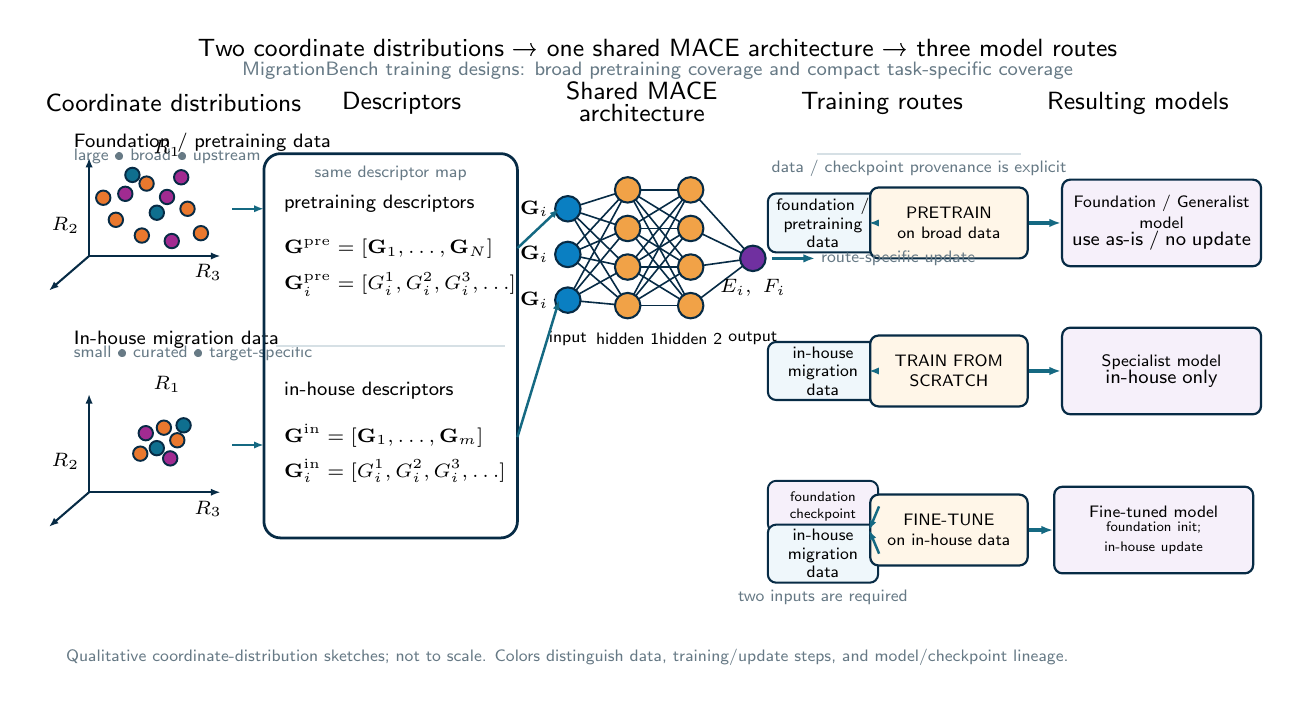
\begin{tikzpicture}[x=0.1mm,y=0.1mm]
  \path[use as bounding box] (0,0) rectangle (1600,850);

  % Overall title and stage titles.
  \node[title] at (800,825) {Two coordinate distributions \textrightarrow{} one shared MACE architecture \textrightarrow{} three model routes};
  \node[subtitle,text=muted] at (800,796) {MigrationBench training designs: broad pretraining coverage and compact task-specific coverage};
  \node[title] at (185,754) {Coordinate distributions};
  \node[title] at (475,754) {Descriptors};
  \node[title] at (780,770) {Shared MACE};
  \node[title] at (780,742) {architecture};
  \node[title] at (1085,754) {Training routes};
  \node[title] at (1410,754) {Resulting models};

  % --------------------------------------------------------------------------
  % Two coordinate-distribution mini-panels.  These are qualitative sketches,
  % not quantitative samples or a performance encoding.
  % --------------------------------------------------------------------------
  \node[subtitle,anchor=west] at (58,704) {Foundation / pretraining data};
  \node[tiny,text=muted,anchor=west] at (58,687) {large \textbullet{} broad \textbullet{} upstream};
  \draw[ink,line width=0.75pt,-{Latex[length=3.5pt,width=2.6pt]}] (78,560) -- (78,685);
  \draw[ink,line width=0.75pt,-{Latex[length=3.5pt,width=2.6pt]}] (78,560) -- (245,560);
  \draw[ink,line width=0.75pt,-{Latex[length=3.5pt,width=2.6pt]}] (78,560) -- (27,516);
  \node[mathlabel] at (48,599) {$R_2$};
  \node[mathlabel] at (177,697) {$R_1$};
  \node[mathlabel] at (229,539) {$R_3$};
  % broad, diffuse cloud
  \node[atom,fill=atomviolet] at (124,639) {};
  \node[atom,fill=atomorange] at (151,652) {};
  \node[atom,fill=atomviolet] at (177,635) {};
  \node[atom,fill=atomorange] at (203,620) {};
  \node[atom,fill=atomorange] at (112,606) {};
  \node[atom,fill=atomorange] at (145,586) {};
  \node[atom,fill=atomviolet] at (183,579) {};
  \node[atom,fill=coordblue] at (164,615) {};
  \node[atom,fill=atomorange] at (220,589) {};
  \node[atom,fill=coordblue] at (133,663) {};
  \node[atom,fill=atomviolet] at (195,660) {};
  \node[atom,fill=atomorange] at (96,634) {};

  \node[subtitle,anchor=west] at (58,454) {In-house migration data};
  \node[tiny,text=muted,anchor=west] at (58,437) {small \textbullet{} curated \textbullet{} target-specific};
  \draw[ink,line width=0.75pt,-{Latex[length=3.5pt,width=2.6pt]}] (78,260) -- (78,385);
  \draw[ink,line width=0.75pt,-{Latex[length=3.5pt,width=2.6pt]}] (78,260) -- (245,260);
  \draw[ink,line width=0.75pt,-{Latex[length=3.5pt,width=2.6pt]}] (78,260) -- (27,216);
  \node[mathlabel] at (48,299) {$R_2$};
  \node[mathlabel] at (177,397) {$R_1$};
  \node[mathlabel] at (229,239) {$R_3$};
  % compact, local cloud
  \node[atom,fill=atomviolet] at (150,335) {};
  \node[atom,fill=atomorange] at (173,342) {};
  \node[atom,fill=atomorange] at (190,326) {};
  \node[atom,fill=coordblue] at (164,316) {};
  \node[atom,fill=atomviolet] at (181,303) {};
  \node[atom,fill=atomorange] at (143,309) {};
  \node[atom,fill=coordblue] at (198,345) {};

  % Separate descriptor rows, fed by the two coordinate sketches.
  \draw[ink,line width=1.0pt,rounded corners=6pt] (300,202) rectangle (622,690);
  \draw[rulegray,line width=0.8pt] (316,446) -- (606,446);
  \node[small,text=muted] at (461,665) {same descriptor map};
  \node[subtitle,anchor=west] at (325,626) {pretraining descriptors};
  \node[mathlabel,anchor=west,font=\rmfamily\fontsize{6.6}{7.6}\selectfont]
    at (325,569) {$\mathbf{G}^{\rm pre}=[\mathbf{G}_1,\ldots,\mathbf{G}_N]$};
  \node[mathlabel,anchor=west,font=\rmfamily\fontsize{6.6}{7.6}\selectfont]
    at (325,524) {$\mathbf{G}^{\rm pre}_i=[G_i^1,G_i^2,G_i^3,\ldots]$};
  \node[subtitle,anchor=west] at (325,389) {in-house descriptors};
  \node[mathlabel,anchor=west,font=\rmfamily\fontsize{6.6}{7.6}\selectfont]
    at (325,332) {$\mathbf{G}^{\rm in}=[\mathbf{G}_1,\ldots,\mathbf{G}_m]$};
  \node[mathlabel,anchor=west,font=\rmfamily\fontsize{6.6}{7.6}\selectfont]
    at (325,287) {$\mathbf{G}^{\rm in}_i=[G_i^1,G_i^2,G_i^3,\ldots]$};
  \thinflow{260,620}{300,620}
  \thinflow{260,320}{300,320}

  % Shared network: connections first, nodes on top.
  \foreach \i in {1,2,3} {
    \foreach \j in {1,2,3,4} {
      \draw[ink,line width=0.58pt] (686,{620-(\i-1)*58}) -- (762,{644-(\j-1)*49});
    }
  }
  \foreach \i in {1,2,3,4} {
    \foreach \j in {1,2,3,4} {
      \draw[ink,line width=0.58pt] (762,{644-(\i-1)*49}) -- (842,{644-(\j-1)*49});
    }
  }
  \foreach \i in {1,2,3,4} {
    \draw[ink,line width=0.58pt] (842,{644-(\i-1)*49}) -- (921,557);
  }
  \foreach \y in {620,562,504} {\node[neuron,fill=inputblue] at (686,\y) {};}
  \foreach \y in {644,595,546,497} {
    \node[neuron,fill=hiddenorange] at (762,\y) {};
    \node[neuron,fill=hiddenorange] at (842,\y) {};
  }
  \node[neuron,fill=outputviolet] at (921,557) {};
  \node[mathlabel,anchor=east] at (662,620) {$\mathbf{G}_i$};
  \node[mathlabel,anchor=east] at (662,562) {$\mathbf{G}_i$};
  \node[mathlabel,anchor=east] at (662,504) {$\mathbf{G}_i$};
  \node[mathlabel] at (921,520) {$E_i,\ F_i$};
  \node[small] at (686,455) {input};
  \node[small] at (762,455) {hidden 1};
  \node[small] at (842,455) {hidden 2};
  \node[small] at (921,455) {output};
  % The two descriptor representations converge on the same architecture.
  \thinflow{622,570}{675,620}
  \thinflow{622,330}{675,504}

  % Training-route panel: equal route weight, explicit route semantics.
  \draw[rulegray,line width=0.8pt] (1002,690) -- (1262,690);
  \node[tiny,text=muted] at (1132,671) {data / checkpoint provenance is explicit};

  % Generalist route.
  \node[datachip] (broad) at (1010,602) {foundation /\\ pretraining\\ data};
  \node[opbox] (pretrain) at (1170,602) {PRETRAIN\\on broad data};
  \thinflow{broad.east}{pretrain.west}
  \node[modelbox] (foundation) at (1440,602) {Foundation / Generalist\\model\\[-1pt]\scriptsize use as-is / no update};
  \mainarrow{pretrain.east}{foundation.west}

  % Specialist route.
  \node[datachip] (indata) at (1010,414) {in-house\\migration\\ data};
  \node[opbox] (scratch) at (1170,414) {TRAIN FROM\\SCRATCH};
  \thinflow{indata.east}{scratch.west}
  \node[modelbox] (specialist) at (1440,414) {Specialist model\\[-1pt]\scriptsize in-house only};
  \mainarrow{scratch.east}{specialist.west}

  % Fine-tuning route: two visibly distinct inputs enter one update box.
  \node[checkpoint] (ckpt) at (1010,242) {foundation\\checkpoint};
  \node[datachip] (target) at (1010,182) {in-house\\migration\\ data};
  \node[opbox] (finetune) at (1170,212) {FINE-TUNE\\on in-house data};
  \thinflow{ckpt.east}{finetune.west}
  \thinflow{target.east}{finetune.west}
  \node[modelbox] (finmodel) at (1430,212) {Fine-tuned model\\[-1pt]\tiny foundation init;\\in-house update};
  \mainarrow{finetune.east}{finmodel.west}
  \node[tiny,text=muted] at (1010,126) {two inputs are required};

  % The shared architecture hands off to the route-specific update panel.
  % The route panel then carries the explicit data/checkpoint inputs itself.
  \mainarrow{945,557}{1000,557}
  \node[tiny,text=muted,anchor=west] at (1007,557) {route-specific update};

  % A compact explanatory note, intentionally non-quantitative.
  \node[tiny,text=muted,anchor=west] at (48,50) {Qualitative coordinate-distribution sketches; not to scale.  Colors distinguish data, training/update steps, and model/checkpoint lineage.};
\end{tikzpicture}
\end{document}
